\documentclass[../master.tex]{subfiles}


\begin{frame}{RStudio: Resources}
\begin{itemize}
	\item RStudio is free and open source;
	\item There are many wonderful cheatsheets at \url{https://www.rstudio.com/resources/cheatsheets/};
	\item A fantastic website showing applications to econometrics with code snippets: \url{https://www.econometrics-with-r.org} (which features also the Card-Krueger example we will look into today).
\end{itemize}
\end{frame}


\begin{frame}[fragile]{Environment}
\begin{itemize}
\item R works with packages. These have to be loaded each time into the workspace with calls of the kind:
\begin{lstlisting}[language=R]
library('')
\end{lstlisting}
\item If you do not have the package on your laptop, you can install any package calling:
\begin{lstlisting}[language=R]
install.packages('')
\end{lstlisting}
with the correct name between quotes;
\item To get help, you can always type a question mark followed by the command that you need help on;
\item Indexing is done with matrix convention (similar to Python, Matlab, etc.) or with a dollar sign for \textit{dataframes}, special data structures that R uses to store data.
\end{itemize}
\end{frame}

\begin{frame}[fragile]{Preliminaries: Working Directory and Libraries}
\begin{itemize}
	\item Define directory with a string
\begin{lstlisting}[language=R]
path='/Users/andreamanera/Dropbox (MIT)/Spring 2019/14-03 Spring 2019 TA Folder/Recitations Spring 2019/Recitation 3 - RStudio/CardKrueger'
outputPath = paste(path,'/out', sep='')
dataPath = paste(path,'/data', sep='')
\end{lstlisting}
\item Set working directory
\begin{lstlisting}[language=R]
setwd(path)
getwd()
\end{lstlisting}
\end{itemize}
\end{frame}


\begin{frame}[fragile]{Manipulating Data with dplyr and foreign}
\begin{itemize}
	\item Import data:
\begin{lstlisting}[language=R] 
data<- read.dta(paste(dataPath, '/fastfood.dta', sep=''))
\end{lstlisting}
This command creates a dataframe in R, a matrix with named columns. Observations (the interviewed restaurants) will be on the rows, while the named columns will denote the variables of interest.
	\item Add variables defined as in CK: for them full time employment is a sum of employees, managers and $.5$ the part time employees
\begin{lstlisting}[language=R]
data <- mutate(data, FTE =  nmgrs + empft + (0.5 * emppt), FTE2 =  nmgrs2 + empft2 + (0.5 * emppt2))
\end{lstlisting}
	\verb|mutate()| generates new data columns using existing ones

\item Can use \verb|subset()| to create smaller datasets of interest (e.g. all restaurants in NJ):
\begin{lstlisting}[language=R]
data_NJ <- data %>% subset(state==1)
\end{lstlisting}
Here we used the pipe operator \verb|%>%| that tells R that it has to use data as an input for subset, i.e. \verb|x %>% f(y)| is equivalent to writing \verb|f(x,y)|.
\end{itemize}
\end{frame}


\begin{frame}[fragile]{Summarize Data}
\begin{itemize}
	\item Use the command \verb|summarize()| that prints a table where the required statistics are stored. e.g. take the means before and after grouping by state:
\begin{lstlisting}[language=R]
data %>% group_by(state) %>% 
   summarize(mean(FTE, na.rm=T),
             mean(FTE2, na.rm=T))
\end{lstlisting}
this prints:
\begin{lstlisting}[language=R]
  state `mean(FTE, na.rm = T)` `mean(FTE2, na.rm = T)`
<int>                  <dbl>                   <dbl>
1     0                   23.3                    21.2
2     1                   20.4                    21.0
\end{lstlisting}
The data reported in the paper. $0$ and $1$ are here the values of the grouping variable state, and recall that $1$ denotes $NJ$.
\item We could have computed the standard deviations using \verb|sd| instead of \verb|mean|.
\end{itemize}
\end{frame}


\section{Testing means}


\subsection{Means and difference of means}
\begin{frame}{How to compare means of two groups?}

\begin{itemize}
	\item Estimate mean for the treatment group \pause
	\[
	\bar{Y}_{X_{i}=1}=\frac{1}{N_{T}}\sum_{i:X_{i}=1}Y_{i}\longrightarrow_{N_{T}\to\infty}E\left[Y_{i}|X_{i}=1\right]
	\]
	
	\item Estimate mean for the control group \pause
	\[
	\bar{Y}_{X_{i}=0}=\frac{1}{N_{C}}\sum_{i:X_{i}=0}Y_{i}\longrightarrow_{N_{C}\to\infty}E\left[Y_{i}|X_{i}=0\right]
	\]
	
	\item Take the difference
	\[
	\hat{d}=\bar{Y}_{X=1}-\bar{Y}_{X=0}\to E\left[Y_{i}|X_{i}=1\right]-E\left[Y_{i}|X_{i}=0\right]
	\]
	
	
	\begin{itemize}
		\item Law of Large Numbers ensures that the estimates are arbitrarily close
		to their population means
	\end{itemize}
\end{itemize}
\end{frame}


\subsection{t-statistics}
\begin{frame}{t-Statistic}

\begin{itemize}
	\item Define a new statistic, the \textbf{t-statistic} as: 
	\[
	t=\frac{\left(\widehat{d}-d\left(=0\right)\right)}{\mbox{se}\left(\hat{d}\right)}
	\]
	
	\item This statistic is approximately normally distributed with mean $0$
	and standard deviation of $1$
	
	\begin{itemize}
		\item exactly normal when sample size is large
	\end{itemize}
\end{itemize}
\end{frame}


\begin{frame}{t-stat (cont...)}


\[
\mathbf{t\mbox{\textbf{-stat:} }}t=\frac{\left(\widehat{d}-d\left(=0\right)\right)}{\mbox{se}\left(\hat{d}\right)}
\]

\begin{itemize}
\item tells us how many standard deviations far is our estimate from the
null (zero)
\item the further from the null it is, the less likely that we got a non-zero
estimate just by random chance 

\end{itemize}

\end{frame}

\begin{frame}{t-stat and p-value}


\begin{center}
\begin{figure}
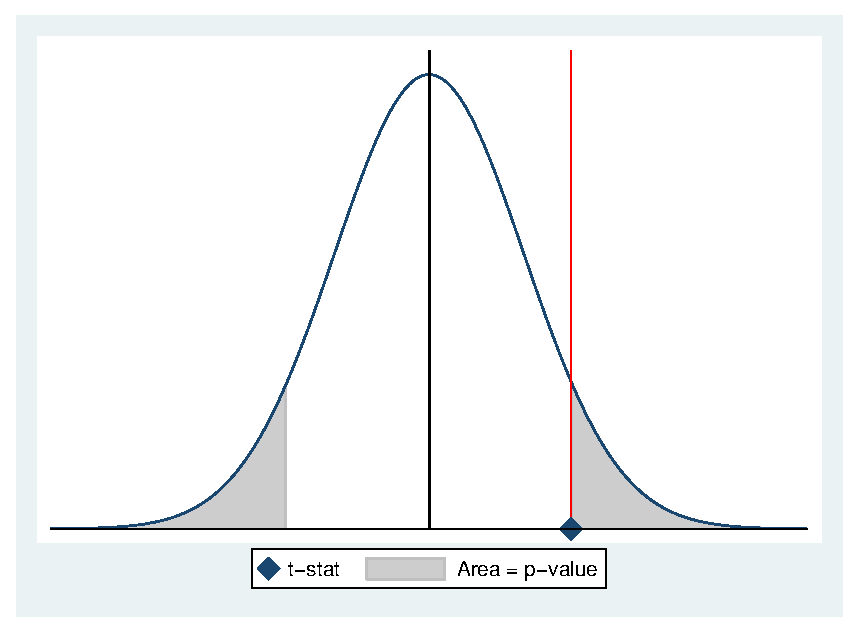
\includegraphics[scale=.6]{tstat.eps}
\end{figure}

\par\end{center}

\end{frame}

\subsection{Hypothesis testing}
\begin{frame}{Hypothesis testing}

\begin{itemize}
\item We want to test the \textbf{Null Hypothesis}: $H_{0}:d=0$ against
the alternative that $H_{a}:d\neq0$

\begin{itemize}
\item The null means (in this case) that the mean of the treatment group
is the same as the mean of the control group. 
\item When treatment is randomly assigned, this is the causal impact of the treatment.
\end{itemize}
\item Suppose that the true value is $d=0$. But since we have a random
sample, it could be that we estimate $\widehat{d}\not=0$ because
of statistical noise (or just by chance) 

\begin{itemize}
\item We want to minimize the chances that we falsely reject the null
\end{itemize}
\item That is, we want to minimize \textbf{Type I Error}: reject the null
when it is actually true
\begin{itemize}
\item We want the probability of making a Type I Error to be low (how low?)
\end{itemize}
\end{itemize}
\end{frame}

\begin{frame}{Statistical Significance }

\begin{itemize}[<+->]
\item To do so, typically adopt a decision rule where if a p-value falls below some threshold $\alpha$ we ``reject" the null.
\item Conventionally, \textbf{statistical significance} $\alpha=0.05$ (5\%). This ensures that we do not make Type-I error mistakes more than $5\%$ of the time.
\item Note the p-value is \textbf{not} the probability of a type-I error. That is, it is not the probability of \textit{incorrectly rejecting} that the null is true.
\item The true interpretation is: the probability that the value of the statistic we observe could be due to sampling error (assuming that Null is true).
In formulas:
\[\text{p-value}=P(\text{Data} |\text{Null is True})\not= P(\text{Null is True}|\text{Data})\]
\item Interestingly, the probability that the Null is true given that the data gave a p-value of $5\%$ can be quite high. See \url{https://faculty.washington.edu/jonno/SISG-2011/lectures/sellkeetal01.pdf} for more information.
\end{itemize}
\end{frame}


\begin{frame}[fragile]{Practically Testing for Difference in Means}
\begin{itemize}
	\item We will use a t-test to see whether the two mean are significantly different in a statistical sense. Our null hypothesis is that their difference is $0$
	\item Carrying out a t-test on R is done through the command \verb|t.test()|. Example: is actual mean number of employees in NJ before the change equal to $20$?
\begin{lstlisting}[language=R]
t.test(data_NJ$FTE, mu=20)
\end{lstlisting}
Turns out it is a good hypothesis \textit{we cannot reject};
The first naive test of the effect of the minimum wage is to see whether there was a significant change in NJ employment after the introduction. To do this we can just compute:
\begin{lstlisting}[language=R]
t.test(data_NJ$FTE,data_NJ$FTE2, mu=0)
\end{lstlisting}
where with \verb|mu=0| we are now testing the hypothesis of no change. It turns out we cannot reject this hypothesis either (the p-value is .42!)

\item But this does not measure anything... other confounding variables might have changed in the meanwhile!

\item \textbf{Diff-in-diff is a potential solution!}
\end{itemize}
\end{frame}

\begin{frame}[fragile]{Diff-in-Diff through a simple t-test}
\begin{itemize}
\item To see how it changed before and after let us build some new variables:
\begin{lstlisting}[language=R]
data %>% mutate(dFTE = FTE2-FTE)
t.test(data_NJ$dFTE, data_PA$dFTE, mu=0, var.equal = T)
\end{lstlisting}	
\item The value of $t$ is very high (larger than the ``magic'' $2$), so we can reject the hypothesis that the difference is $0$, in favor of a positive effect of the minimum wage;
\item \verb|var.equal| tells R to use the all observations to compute the variance instead of treating the two sets of observations for PA and NJ as coming from different samples. (see commands in \hyperlink{regslide}{\beamerbutton{Slide with Regression}}\hypertarget{ttest})
\item This replicates Table 3, column (iii) in CK (1994).
\end{itemize}
\end{frame}




\begin{frame}{Means}

\begin{itemize}
	\item We can also accomplish similar objectives using regression
	\item Suppose you have data $\left(y_{i}\right)$ that you are interested
	in
	\item You can always write this as 
	\[
	y_{i}=\alpha+\varepsilon_{i}
	\]
	where $E\left[\varepsilon_{i}\right]=0$, then
	\[
	E\left[y_{i}\right]=\alpha
	\]
	\pause
	\item Suppose you wanted to see the means by two groups $X_{i}=1$ and $X_{i}=0$
	\item Similarly you can write, for $X_{i}=0$ 
	\[
	y_{i}=\alpha+\varepsilon_{i}\mbox{ with }E\left[\varepsilon_{i}|X_{i}=0\right]=0
	\]
	and for $X_{i}=1$
	\[
	y_{i}=\alpha+\beta+\eta_{i}\mbox{ with }E\left[\eta_{i}|X_{i}=1\right]=0
	\]
	
\end{itemize}
\end{frame}

\begin{frame}{Comparing means in two group}

\begin{itemize}
\item Combining, we get
\[
y_{i}=\alpha+\beta X_{i}+\epsilon_{i}
\]
with $E\left[\epsilon_{i}|X_{i}\right]=0$
\item Since $E\left[\varepsilon_{i}|X_{i}=0\right]=E\left[\eta_{i}|X_{i}=1\right]=0$,
we have 
\[
\begin{aligned}E\left[y_{i}|X_{i}=1\right]= & \alpha+\beta\\
E\left[y_{i}|X_{i}=0\right]= & \alpha
\end{aligned}
\implies E\left[y_{i}|X_{i}=1\right]-E\left[y_{i}|X_{i}=0\right]=\beta
\]

\item How do we implement this? 
\end{itemize}
\end{frame}

\begin{frame}{Comparing means in multiple groups}

\begin{itemize}
\item Can similar think of the situation where there are many groups. Let
$X0_{i},X1_{i},X2_{i},\cdots,Xk_{i}$ indicate the $k+1$ groups.
Then can write
\[
y_{i}=\alpha+\beta_{1}X1_{i}+\beta_{2}X2_{i}+\cdots+\beta_{k}Xk_{i}+\varepsilon_{i}
\]
with $E\left[\varepsilon_{i}|X_{i}\right]=0$. (note the omission
of $X0_{i}$) 
\item Then
\[
\begin{aligned}\beta_{1}= & E\left[y_{i}|X1_{i}=1\right]-E\left[y_{i}|X0_{i}=1\right]\\
\beta_{2}= & E\left[y_{i}|X2_{i}=1\right]-E\left[y_{i}|X0_{i}=1\right]\\
& \vdots\\
\beta_{k}= & E\left[y_{i}|Xk_{i}=1\right]-E\left[y_{i}|X0_{i}=1\right]
\end{aligned}
\]

\item How do we compare group $j$ with group $k$? 
\item How do we estimate the $\beta$s?
\end{itemize}
\end{frame}

\begin{frame}{Regression}

\begin{itemize}
\item Regression can estimate the following relationships
\[
y_{i}=\alpha+\beta X_{i}+\varepsilon_{i}
\]
\[
y_{i}=\alpha+\beta_{1}X1_{i}+\beta_{2}X2_{i}+\cdots+\beta_{k}Xk_{i}+\varepsilon_{i}
\]
with $E\left[\varepsilon_{i}|X_{i}\right]=0$
\item Ordinary Least Squares (OLS) is the best linear unbiased estimator of coefficients
\item Can then conduct many hypothesis tests of interest
\end{itemize}
\end{frame}

\begin{frame}
\frametitle{Testing Treatment}

\begin{itemize}
\item One of the most common versions we're interested in is 
\[y_i=\alpha+\beta X_i+\epsilon_i\]
where $X_i$ is an indicator variable for being treated.
\item As noted this then gives us $\beta=E[Y|X=1]-E[Y|X=0]$ or the treatment effect.
\end{itemize}
\end{frame}

\section{Testing linear relationships}


\subsection{Setup}
\begin{frame}{Testing linear relationships}

\begin{itemize}
\item We can also use OLS to test whether two variables of economic
interest are related to each other
\item We have our data in two variables 
\[
y=\left(y_{1},y_{2},...,y_{N}\right)
\]
\[
x=\left(x_{1},x_{2},...,x_{N}\right)
\]


\begin{itemize}
\item $y$ is the dependent variable (say FTE employment)
\item $x$ is the explanatory variable/ exogenous variable (say a dummy for ``minimum wage introduced'')
\end{itemize}
\item Write the simplest relationship between the two variables
\[
E\left[y|x\right]=a+bx
\]

\item Best linear approximation of $E[Y|X]$
\end{itemize}
\end{frame}



\begin{frame}[fragile]{Practically Using Regressions for CK (1994)}
\begin{itemize}
	\item Running Regressions can be done specifying a model using the command \verb|lm| (which stands for ``linear model'').
	\item First reorganize the data to make it ``long'' from its current ``wide'' form
\begin{lstlisting}[language=R]
#Create dataframe with employment before the change
dataBefore <- data.frame(id = data$sheet,
chain = data$chain,
state = data$state, 
empl = data$FTE) %>% 
mutate(after = 0)
#Create dataframe with employment after the change
dataAfter <- data.frame(id = data$sheet,
chain = data$chain,
state = data$state,
empl = data$FTE2) %>% 
mutate(after = 1)
#Concatenate vertically
dataReg <- data.frame(rbind(dataBefore, dataAfter))
\end{lstlisting}	
\end{itemize}

\end{frame}


\begin{frame}[fragile]{Step 1: ``Naive Regression''}
\begin{itemize}
	\item Run a regression on data from NJ only before and after the introduction of the minimum wage. Our model is:
	\[Empl_{i,t} = \alpha + \beta\mathbf{1}(W_{min} \ \text{introduced for $i$})   \]
	($i$ denotes the restaurant).
	\item In R:
\begin{lstlisting}[language=R]
### Specify the naive model of interest
model <- lm(formula = empl ~ after,
data =dataReg,
subset = 
(dataReg$state == 1))
\end{lstlisting}	
\item \verb|formula| denotes our model, constant $\alpha$ is always included by default. \verb|subset| allows us to run the regression on a subset.	
\end{itemize}
\end{frame}

\begin{frame}[fragile]{Step 1.1: Testing Coefficients}
\begin{itemize}
	\item Testing in R takes as input a model of the kind we defined before. The function to get diagnostics is \verb|coeftest| in the package \verb|AER| (so we need to call \verb|library(AER)| before). To see diagnostic for the naive regression:
\begin{lstlisting}[language=R]
coeftest(model, vcov. = vcovHC, type = "HC1")
\end{lstlisting}
Options are technical (if you have heard of heteroskedasticity, these are used to get heteroskedasticity-robust standard errors).
\item Output:
\begin{lstlisting}[language=R]
t test of coefficients:

Estimate Std. Error t value Pr(>|t|)    
(Intercept) 20.43941    0.50826 40.2142   <2e-16 ***
after        0.58802    0.72736  0.8084   0.4191    
---
Signif. codes:  0 ‘***’ 0.001 ‘**’ 0.01 ‘*’ 0.05 ‘.’ 0.1 ‘ ’ 1
\end{lstlisting}
We see there is no statistical significance on ``after''. What can we conclude?
\item Actually, nothing at all!
\end{itemize}
\end{frame}



\begin{frame}[fragile]{Step 2: The Regression in Recitation}
\begin{itemize}
	\item Run a regression on data from both states. Our model becomes:
	\begin{align*}
		Empl_{i,t} &= \alpha + \beta_1\mathbf{1}_{i,t}(W_{min} \ \text{introduced}) +\beta_2\mathbf{1}_{i,t}(\text{State $=$ NJ})+\\ &+ \beta_{3}\mathbf{1}_{i,t}(W_{min} \ \text{introduced})\mathbf{1}_{i,t}(\text{State $=$ NJ}) 
	\end{align*}
	\item $\beta_3$ is the diff-in-diff coefficient.
\begin{lstlisting}[language=R]
### Specify the CK model of interest and get diagnostics
modelCK <- lm(formula = empl ~ state*after,
data =dataReg)
coeftest(modelCK, vcov. = vcovHC, type = "HC1")
\end{lstlisting}	
	\item \verb|formula| denotes our model, constant $\alpha$ is always included by default. \verb|subset| allows us to run the regression on a subset.	
\end{itemize}
\end{frame}


\begin{frame}[fragile]{Step 3: The Card-Krueger Regression}
\begin{itemize}
	\item We can take differences over time so that the model
	\begin{align*}
	Empl_{i,t} &= \alpha + \beta_1\mathbf{1}_{i,t}(W_{min} \ \text{introduced}) +\beta_2\mathbf{1}_{i,t}(\text{State $=$ NJ})+\\ &+ \beta_{3}\mathbf{1}_{i,t}(W_{min} \ \text{introduced})\mathbf{1}_{i,t}(\text{State $=$ NJ}) 
	\end{align*}
	becomes (convince yourself taking the differences along the time dimension):
	\begin{align*}
	\Delta Empl_{i,1} = Empl_{i,1} - Empl_{i,0}  &=  \beta_1 +\beta_3\mathbf{1}_{i,1}(\text{State $=$ NJ})
	\end{align*}
	\item $\beta_3$ is the diff-in-diff coefficient.
\begin{lstlisting}[language=R]
### Specify the CK model of interest and get diagnostics
modelDiff = lm(formula = dFTE ~ state, data = data)
coeftest(modelDiff)
\end{lstlisting}	
	\item You will see that the t-tstat is the same as the one we obtained at the beginning (rerun the command in \hyperlink{ttest}{\beamerbutton{Slide on t-test}} \hypertarget{regslide}{})
\end{itemize}
\end{frame}


\begin{frame}[fragile]{Step 3: Replicating Table 4 in CK (1994)}
\begin{itemize}
\item Note that CK do not get 2.75 as coefficient in Table 4, column 1, but 2.33. This is because they select the sample to include only observations with wages in both years
\item To carry out the sample selection, we need to drop observations that are \verb|NA|. This is achieved as follows:
\begin{lstlisting}[language=R]
dataAllWages = data[complete.cases(
data.frame(data$wage_st,data$wage_st2, data$FTE, data$FTE2)),]
\end{lstlisting}
\item \verb|complete.cases| identifies the rows of the dataset in parentheses that contain \textit{no missing values}. This produces logical indexes that are then used to select the rows of \verb|data| (convince yourself this works).
\begin{lstlisting}[language=R]
modelDiff = lm(formula = dFTE ~ state, data = dataAllWages)
coeftest(modelDiff)
\end{lstlisting}
produces a coefficient of $2.28$, very close to the $2.33$ obtained by CK, and the same standard error. The difference is explained by the sample: if we follow their indications we get a sample of $359$ observations, not $357$ as they say...
\item Many times economic papers do not exactly replicate!
\end{itemize}
\end{frame}



\begin{frame}{Extra: Diff-in-Diff with graphs I}
\centering
\includegraphics[scale=.45]{Trends.png}
\end{frame}

\begin{frame}{Extra: Diff-in-Diff with graphs II}
\centering
\includegraphics[scale=.45]{DiffInDiffLines.png}
\end{frame}

\begin{frame}{Extra: Diff-in-Diff with graphs III}
\centering
\includegraphics[scale=.45]{DiffInDiffOnlyLines.png}
\end{frame}






